\chapter{Experimental part: Data cleaning}
\label{chap:clean}
In this chapter, we will present the process of the raw dataset cleaning. As we discussed in previous chapters, we extracted raw web features separately for event components (name, date, location, description) and for random elements of the page. We aim to construct train dataset with both positive and negative examples for every event component to build binary classifiers. \\

This chapter opens the block of the chapters which cover the Experimental part of the thesis. We will often refer to the Python code which may be found in corresponding Jupyter notebooks. In this chapter, we cover the main stages and present the scheme of the whole cleaning pipeline. Also we will show how the raw data is melting, meaning after the every step of the cleaning process the amount of data is reducing dramatically. The less important results will be available in Appendix chapter. The whole process together with the corresponding code you may see in the notebooks with the prefix \textit{Clean}.\\

The process of big dataset cleaning usually is very time-consuming and in our thesis, it was not an exception. The reason for this in our case is that the dataset is basically artificial and collected from the Internet by our crawlers. During the collecting stage, we could face problems with the web element availability, encoding, duplicates, missing values and all other natural effects. We separated the whole process into 4 logical components. The the first component we remove the rows which have an obvious damage. In the second component we look closer and work specifically with the CSS properties since there are more than 200 features and not all of them are relevant for us. In the third part, we work with \textit{frequent domains} which have a lot of similar URL pages. In the last part, we work with the outliers and logically not-existing values of the features. \\

On the picture \nameref{fig:clean} you main see the main stages of the cleaning process.

\begin{figure}[h]
\begin{center}
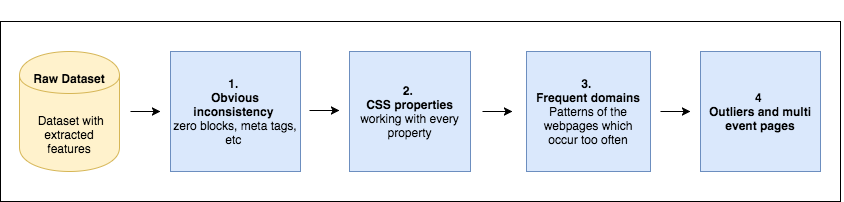
\includegraphics[width=1.0\textwidth]{figures06/clean_workflow1}
\caption{Raw data-cleaning workflow}
\label{fig:clean}
\end{center}
\end{figure}

Let's discuss every part of this schema.\\

\section*{Obvious inconsistency}

Here we worked with several types of inconsistency:

\begin{itemize}
    \item 
\end{itemize}

